\documentclass[tikz]{standalone} 
% change to font used in beamer
%\renewcommand{\familydefault}{\sfdefault}

\usetikzlibrary{patterns}

\begin{document}
	
	\newlength{\scale}
	\setlength{\scale}{30pt}
	
	%\tdplotsetmaincoords{0}{0}
	\begin{tikzpicture}[scale=1.5]
		
		\node[inner sep=0pt] (plot) at (0,0)
		{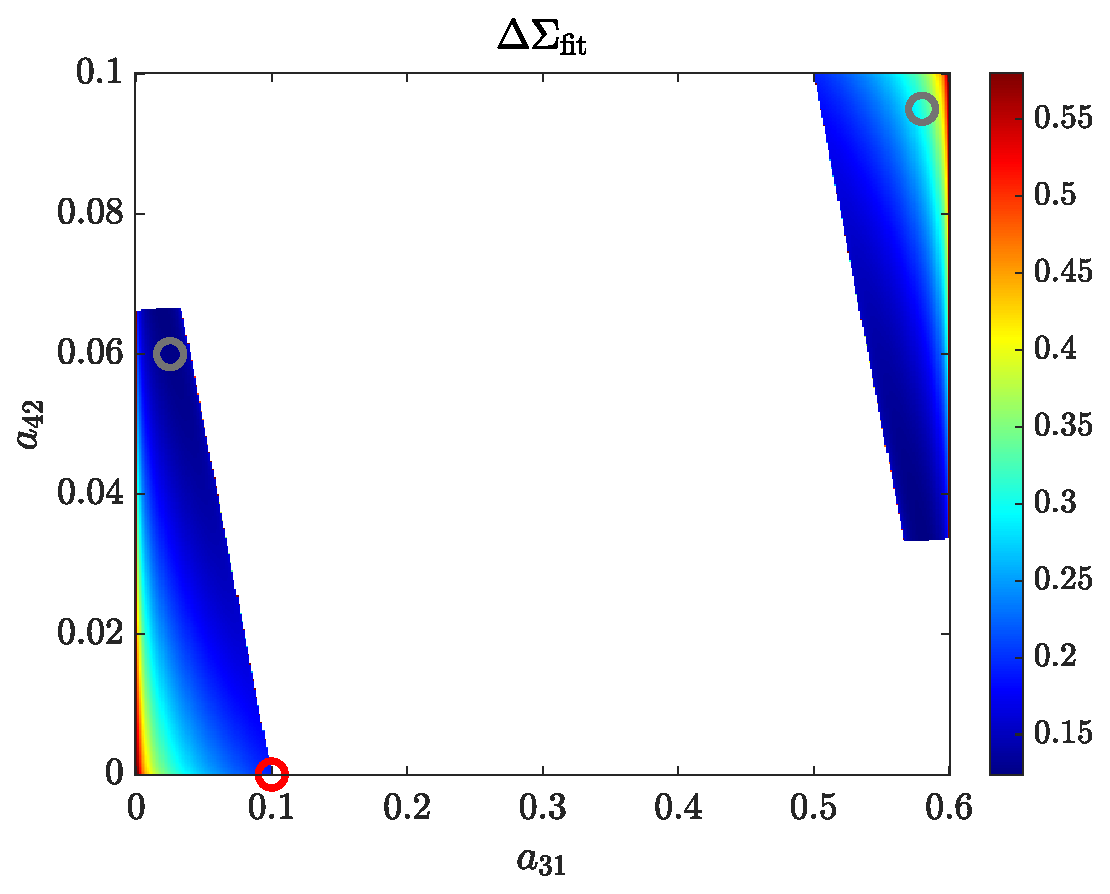
\includegraphics[width=7cm]{EP_est_free_parameters.eps}};
		
		% Network 1 (upper right)
		\begin{scope}[shift={(2.9,1.1)}]
			\draw[very thick,gray] (0.5,-0.5) to (-1.25,0.34);
			\draw[very thick,gray,fill=white] (0.5,-0.5) circle (1);
			
			\draw[ultra thick,fill=white] (0,0) circle (0.18) node[]{$1$};
			\draw[ultra thick,fill = white] (1,0) circle (0.18) node[]{$2$};
			\fill[gray] (0,-1) circle (0.18);
			\fill[gray] (1,-1) circle (0.18);
			% j_21
			\draw[line width = 0.0108\scale,<-,blue!50!black] (0.23,0) to (0.77,0);
			% j_31
			\draw[line width = 0.0812\scale,->,blue!50!black] (0.163,-0.163) to (0.837,-0.837);
			% j_41
			\draw[line width = 0.0704\scale,<-,blue!50!black] (0,-0.23) to (0,-0.77);
			% j_32
			\draw[line width = 0.0027\scale,<-,blue!50!black] (1,-0.23) to (1,-0.77);
			% j_42
			\draw[line width = 0.0081\scale,<-,blue!50!black] (0.837,-0.163) to (0.163,-0.837);
			% j_43
			\draw[line width = 0.0785\scale,->,blue!50!black]  (0.77,-1) to (0.23,-1);
		\end{scope}
		
		% Network 2 (upper left)
		\begin{scope}[shift={(-3.7,1.5)}]
			\draw[very thick,gray] (0.5,-0.5) to (1.98,-1.08);
			\draw[very thick,gray,fill=white] (0.5,-0.5) circle (1);
			
			\draw[ultra thick,fill=white] (0,0) circle (0.18) node[]{$1$};
			\draw[ultra thick,fill = white] (1,0) circle (0.18) node[]{$2$};
			\fill[gray] (0,-1) circle (0.18);
			\fill[gray] (1,-1) circle (0.18);
			% j_21
			\draw[line width = 0.0108\scale,<-,blue!50!black] (0.23,0) to (0.77,0);
			% j_31
			\draw[line width = 0.0273\scale,<-,blue!50!black] (0.163,-0.163) to (0.837,-0.837);
			% j_41
			\draw[line width = 0.0381\scale,->,blue!50!black] (0,-0.23) to (0,-0.77);
			% j_32
			\draw[line width = 0.0196\scale,<-,blue!50!black] (1,-0.23) to (1,-0.77);
			% j_42
			\draw[line width = 0.0088\scale,->,blue!50!black] (0.837,-0.163) to (0.163,-0.837);
			% j_43
			\draw[line width = 0.0469\scale,<-,blue!50!black]  (0.77,-1) to (0.23,-1);
		\end{scope}
		
		% generating Network
		\begin{scope}[shift={(-0.55,0.16)}]
			\draw[very thick,red] (0.5,-0.5) to (-0.63,-1.54);
			\draw[very thick,red,fill=white] (0.5,-0.5) circle (1);
			
			\draw[ultra thick,fill=white] (0,0) circle (0.18) node[]{$1$};
			\draw[ultra thick,fill = white] (1,0) circle (0.18) node[]{$2$};
			\fill[gray] (0,-1) circle (0.18);
			\fill[gray] (1,-1) circle (0.18);
			% j_21
			\draw[line width = 0.0108\scale,<-,blue!50!black] (0.23,0) to (0.77,0);
			% j_31
			\draw[line width = 0.0626\scale,<-,blue!50!black] (0.163,-0.163) to (0.837,-0.837);
			% j_41
			\draw[line width = 0.0734\scale,->,blue!50!black] (0,-0.23) to (0,-0.77);
			% j_32
			\draw[line width = 0.0108\scale,<-,blue!50!black] (1,-0.23) to (1,-0.77);
			% j_42
			%\draw[line width = 0\scale,->,blue!50!black] (0.837,-0.163) to (0.163,-0.837);
			% j_43
			\draw[line width = 0.0734\scale,<-,blue!50!black]  (0.77,-1) to (0.23,-1);
		\end{scope}
		
	\end{tikzpicture}
	
\end{document}